\documentclass[border=10pt]{standalone}
\usepackage[utf8]{inputenc}
\usepackage{tikz}
\usetikzlibrary{positioning, shadows, arrows.meta, fit, backgrounds}
\usepackage{amssymb}

\begin{document}
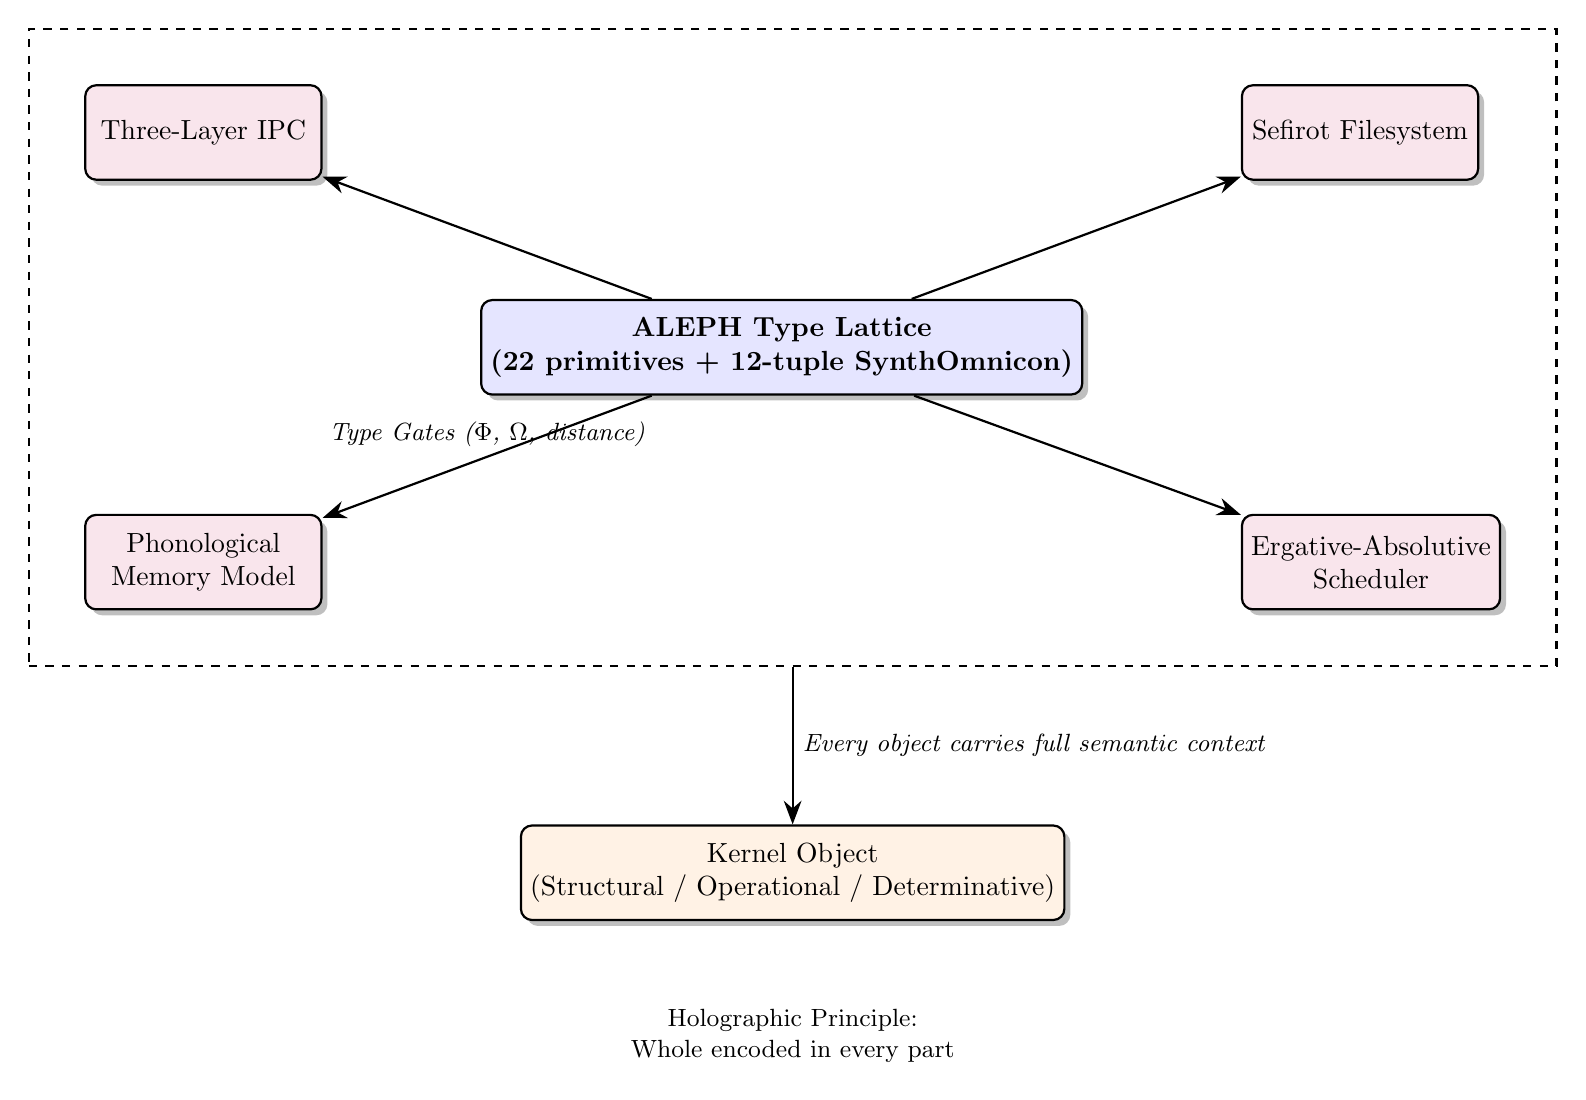
\begin{tikzpicture}[
    node distance=1.5cm and 2cm,
    box/.style={rectangle, draw, thick, rounded corners, minimum width=3cm, minimum height=1.2cm, align=center, drop shadow},
    core/.style={box, fill=blue!10, font=\bfseries},
    sub/.style={box, fill=purple!10},
    arrow/.style={-{Stealth[length=3mm]}, thick},
    label/.style={font=\small\itshape}
]

% Central ALEPH Core
\node[core] (aleph) {ALEPH Type Lattice\\(22 primitives + 12-tuple SynthOmnicon)};

% Subsystems
\node[sub, below left=of aleph] (mem) {Phonological\\Memory Model};
\node[sub, below right=of aleph] (sched) {Ergative-Absolutive\\Scheduler};
\node[sub, above left=of aleph] (ipc) {Three-Layer IPC};
\node[sub, above right=of aleph] (fs) {Sefirot Filesystem};

% Kernel objects wrapper
\node[fit=(mem)(sched)(ipc)(fs)(aleph), draw, dashed, thick, inner sep=20pt, label=above:Holographic Kernel] (kernel) {};

% Three-layer objects (example)
\node[box, fill=orange!10, below=2cm of kernel] (obj) {Kernel Object\\(Structural / Operational / Determinative)};

% Connections with type gates
\draw[arrow] (aleph) -- (mem) node[midway, label, above] {Type Gates ($\Phi$, $\Omega$, distance)};
\draw[arrow] (aleph) -- (sched);
\draw[arrow] (aleph) -- (ipc);
\draw[arrow] (aleph) -- (fs);
\draw[arrow] (kernel.south) -- (obj.north) node[midway, label, right] {Every object carries full semantic context};

% Holographic note
\node[align=center, below=1cm of obj, font=\small] {Holographic Principle: \\ Whole encoded in every part};

\end{tikzpicture}
\end{document}
